\section{Resource allocation for a system following a pipe and filter like architecture}
This section focuses on the main challenges of implementing resource allocation without losing fault tolerance or decoupling between components. Replicas of the same component have no means of organizing, they just take the next job that is available in the queue and execute it, no mechanism for distributing the jobs is in place. Replicas of the same component can consume different amounts of system resources, depending on the type of job they are executing, bat because they have no possibility to select the jobs they will execute, they just take the next job from the queue, we cannot predict on which of the replicas the job will be executed. Because of this unpredictability, the task of allocating resources becomes challenging and different methods have been proposed.

\subsection{Method 1: Allows the system to balance work in a natural way and not intervene in job allocation}
Fig. \ref{fig:randomDIstributionsOfTasks}

\begin{figure}[ht]
\centering
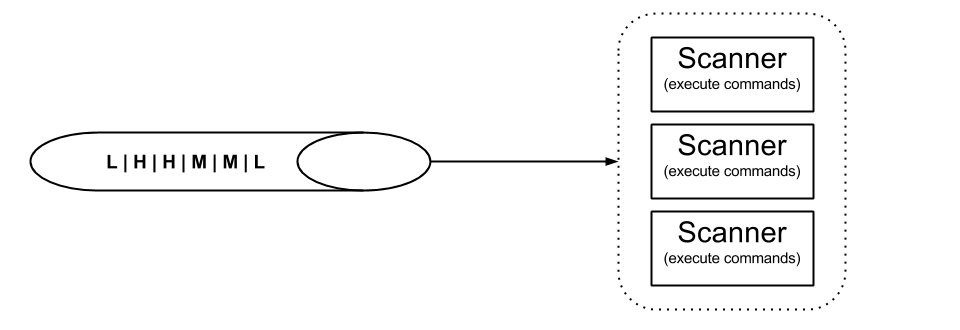
\includegraphics[width=\linewidth]{./img/1_NaturalLoadBalancing.png}
\caption{Random distribution of tasks}
\label{fig:randomDIstributionsOfTasks}
\end{figure}

\subsection{Method 2: Assign sizes to jobs and constrain component replicas to execute some type of jobs with a higher priority than others}

\subsection{Method 3: Create multiple queues deepening on the size of the jobs}

\subsection{Method 4: Use other types of data structure to send the jobs from one component to another}
